%%%%%%%%%%%%%%%%%%%%%%%%%%%%%%%%%%%%%%%%%%%%%%%%%%%%%%%%%%%%%%%
%
% Welcome to Overleaf --- just edit your LaTeX on the left,
% and we'll compile it for you on the right. If you open the
% 'Share' menu, you can invite other users to edit at the same
% time. See www.overleaf.com/learn for more info. Enjoy!
%
%%%%%%%%%%%%%%%%%%%%%%%%%%%%%%%%%%%%%%%%%%%%%%%%%%%%%%%%%%%%%%%
% How to Draw Flowcharts in LaTeX using TikZ?
% latexdraw.com
% 30/01/2021 at 00:07

\documentclass[border=0.2cm]{standalone}

% Required packages
\usepackage{tikz}
\usetikzlibrary{shapes,positioning}
\usepackage{makecell}
\usepackage{pgfplots}
\tikzstyle{arrow}=[draw]
\tikzstyle{arrow}=[draw, -latex]

\begin{document}

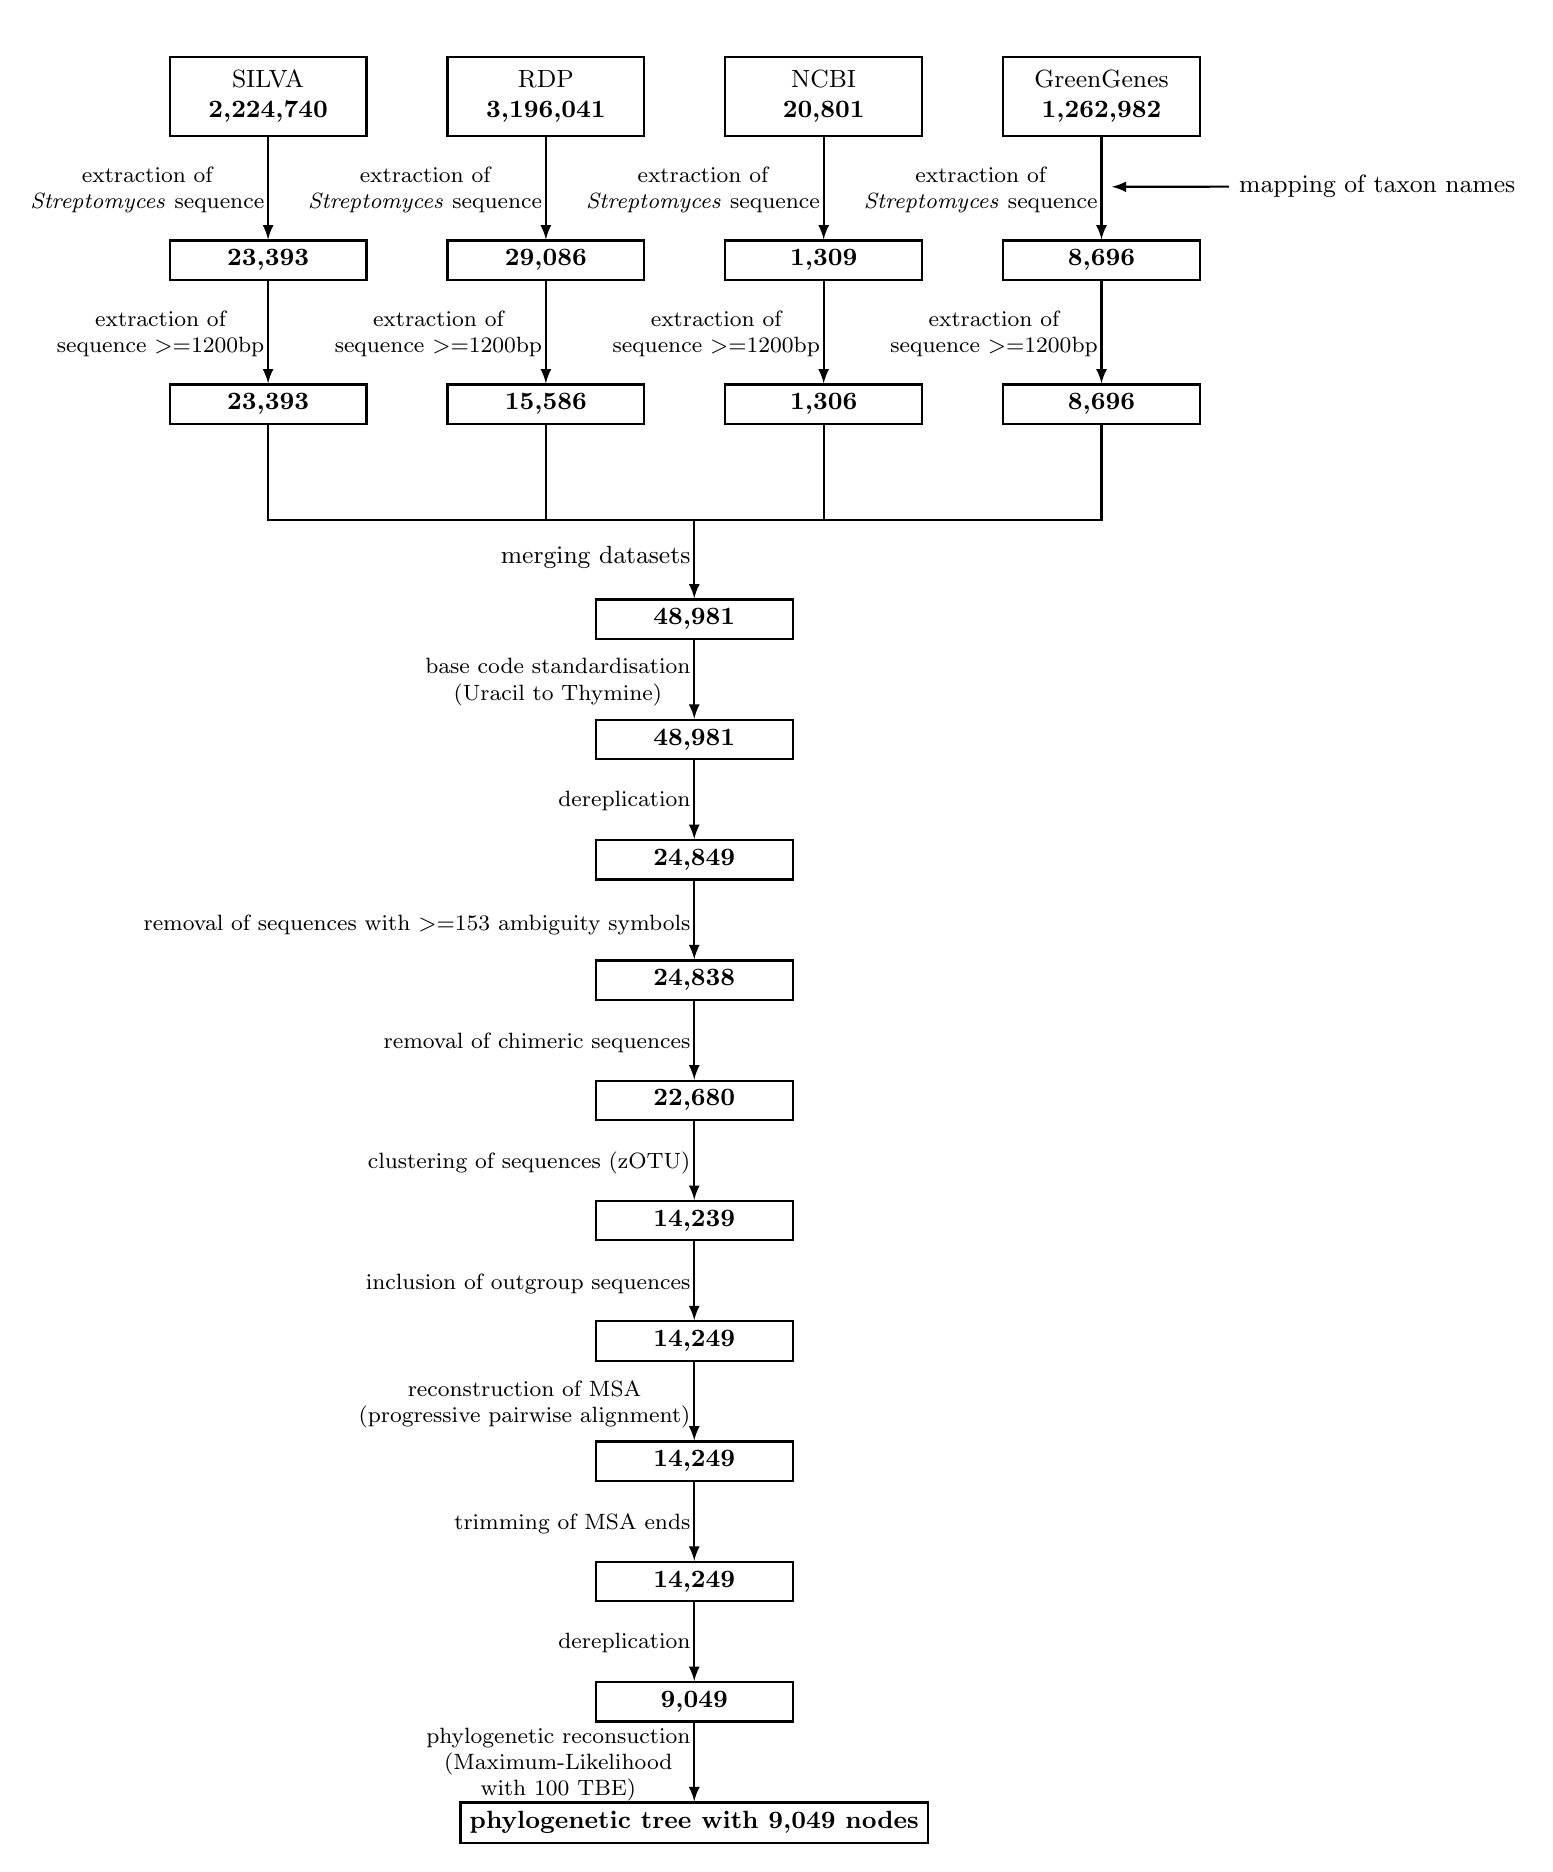
\begin{tikzpicture}[font=\small,thick]



% Conditions test
\node[
    left = 3cm,
    minimum width=1cm] (block15){};

\node[draw,
    below left=0.15cm of block15,
    minimum width=2.5cm] (block4){\makecell[ct]{RDP\\ \textbf{3,196,041}}};


\node[draw,
    left=of block4,
    minimum width=2.5cm] (block16){\makecell[ct]{SILVA\\ \textbf{2,224,740}}};

\node[draw,
    right=of block4,
    minimum width=2.5cm] (block17){\makecell[ct]{NCBI\\ \textbf{20,801}}};

\node[draw,
    right=of block17,
    minimum width=2.5cm] (block18){\makecell[ct]{GreenGenes\\ \textbf{1,262,982}}};


\node[draw,
    below=1.3cm of block4,
    minimum width=2.5cm] (block1) {\textbf{29,086}};


\node[draw,
    left=of block1,
    minimum width=2.5cm] (block2) {\textbf{23,393}};

\node[draw,
    below=1.3cm of block17,
    minimum width=2.5cm] (block6) {\textbf{1,309}};

\node[draw,
    right=of block6,
    minimum width=2.5cm] (block3) {\textbf{8,696}};

\node[
    below right=0.5cm of block18,
    minimum width=0.5cm] (block5) {mapping of taxon names};

\node[
    below =0.5cm of block18,
    minimum width=0.001cm] (block0) { };

% Increase and Decrease duty cycle
\node[draw,
    below=1.3cm of block1,
    minimum width=2.5cm] (block7){\textbf{15,586}};

\node[draw,
    left=of block7,
    minimum width=2.5cm] (block8){\textbf{23,393}};

\node[draw,
    align=center,
    below=1.3cm of block6,
    minimum width=2.5cm] (block9){\textbf{1,306}};

\node[draw,
    right=of block9,
    minimum width=2.5cm] (block10){\textbf{8,696}};

% Return block
\node[draw,
    below=7cm of block15,
    minimum width=2.5cm] (block11)  {\textbf{48,981}};

\node[coordinate,below=6cm of block15] (block12) {Block 12};

\node[draw,
    below=of block11,
    minimum width=2.5cm] (block13){\textbf{48,981}};

\node[draw,
    below=of block13,
    minimum width=2.5cm] (block19){\textbf{24,849}};

\node[draw,
    below=of block19,
    minimum width=2.5cm] (block20){\textbf{24,838}};

\node[draw,
    below=of block20,
    minimum width=2.5cm] (block21){\textbf{22,680}};

\node[draw,
    below=of block21,
    minimum width=2.5cm] (block22){\textbf{14,239}};

\node[draw,
    below=of block22,
    minimum width=2.5cm] (block23){\textbf{14,249}};

\node[draw,
    below=of block23,
    minimum width=2.5cm] (block24){\textbf{14,249}};

\node[draw,
    below=of block24,
    minimum width=2.5cm] (block25){\textbf{14,249}};

\node[draw,
    below=of block25,
    minimum width=2.5cm] (block26){\textbf{9,049}};

\node[draw,
    below=of block26,
    minimum width=2.5cm] (block27){\textbf{phylogenetic tree with 9,049 nodes}};



% Arrows

\draw (block7) |- (block12);
\draw (block9) |- (block12);
\draw (block8) |- (block7|-block12);
\draw (block10) |- (block9|-block12);
\draw[-latex] (block12) -- (block11) node[pos=0.5,anchor=-1,inner sep=1pt]{merging datasets};

\draw[-latex] (block16) -- (block2) node[pos=0.5,anchor=1,inner sep=1pt]{\footnotesize  {\makecell[ct]{extraction of \\ \textit{Streptomyces} sequence }}};

\draw[-latex] (block4) -- (block1) node[pos=0.5,anchor=1,inner sep=1pt]{\footnotesize  {\makecell[ct]{extraction of \\ \textit{Streptomyces} sequence }}};

\draw[-latex] (block17) -- (block6) node[pos=0.5,anchor=1,inner sep=1pt]{\footnotesize  {\makecell[ct]{extraction of \\ \textit{Streptomyces} sequence }}};

\draw[-latex] (block18) -- (block3) node[pos=0.5,anchor=1,inner sep=1pt]{\footnotesize  {\makecell[ct]{extraction of \\ \textit{Streptomyces} sequence }}};

\draw[-latex] (block2) -- (block8) node[pos=0.5,anchor=1,inner sep=1pt]{\footnotesize  {\makecell[ct]{extraction of \\sequence $>=$1200bp}}};

\draw[-latex] (block1) -- (block7) node[pos=0.5,anchor=1,inner sep=1pt]{\footnotesize  {\makecell[ct]{extraction of \\sequence $>=$1200bp}}};

\draw[-latex] (block6) -- (block9) node[pos=0.5,anchor=1,inner sep=1pt]{\footnotesize  {\makecell[ct]{extraction of \\sequence $>=$1200bp}}};

\draw[-latex] (block3) -- (block10) node[pos=0.5,anchor=1,inner sep=1pt]{\footnotesize  {\makecell[ct]{extraction of \\sequence $>=$1200bp}}};

\draw[-latex] (block11) -- (block13) node[pos=0.5,anchor=1,inner sep=1pt]{\footnotesize  {\makecell[ct]{base code standardisation \\ (Uracil to Thymine)}}};


\draw[-latex] (block5) -- (block0) node[pos=0.5,anchor=1,inner sep=1pt]{};

\draw[-latex] (block13) -- (block19) node[pos=0.5,anchor=1,inner sep=1pt]{\footnotesize dereplication};

\draw[-latex] (block19) -- (block20) node[pos=0.5,anchor=1,inner sep=1pt]{\footnotesize removal of sequences with $>=$153 ambiguity symbols};

\draw[-latex] (block20) -- (block21) node[pos=0.5,anchor=1,inner sep=1pt]{\footnotesize removal of chimeric sequences};

\draw[-latex] (block21) -- (block22) node[pos=0.5,anchor=1,inner sep=1pt]{\footnotesize clustering of sequences (zOTU)};

\draw[-latex] (block22) -- (block23) node[pos=0.5,anchor=1,inner sep=1pt]{\footnotesize inclusion of outgroup sequences};

\draw[-latex] (block23) -- (block24) node[pos=0.5,anchor=1,inner sep=1pt]{\footnotesize  {\makecell[ct]{reconstruction of MSA \\ (progressive pairwise alignment)}}};


{\footnotesize reconstruction of MSA \\ (progressive pairwise alignment)};

\draw[-latex] (block24) -- (block25) node[pos=0.5,anchor=1,inner sep=1pt]{\footnotesize trimming of MSA ends};

\draw[-latex] (block25) -- (block26) node[pos=0.5,anchor=1,inner sep=1pt]{\footnotesize dereplication};

\draw[-latex] (block26) -- (block27) node[pos=0.5,anchor=1,inner sep=1pt]{\footnotesize  {\makecell[ct]{phylogenetic reconsuction \\ (Maximum-Likelihood \\ with 100 TBE)}}};

\end{tikzpicture}

\end{document}